%\begin{landscape}

\chapter{Programa}

% These set the width of a day and the height of an hour.
%\newcommand*\daywidth{4.5cm}
%\newcommand*\hourheight{3em}

\newcommand*\daywidth{3.4cm}
\newcommand*\hourheight{3em}

% The entry style will have two options:
% * the first option sets how many hours the entry will be (i.e. its height);
% * the second option sets how many overlapping entries there are (thus
%   determining the width).
\tikzset{entry/.style 2 args={
    xshift=(0.5334em+0.8pt)/2,
    draw,
    line width=1pt,
    font=\sffamily,
    rectangle,
    rounded corners,
    fill=white,
    anchor=north west,
    inner sep=0.1em,
    text width={\daywidth/#2-0.85em},
    minimum height=#1*\hourheight,
    align=center
}}

% Start the picture and set the x coordinate to correspond to days and the y
% coordinate to correspond to hours (y should point downwards).
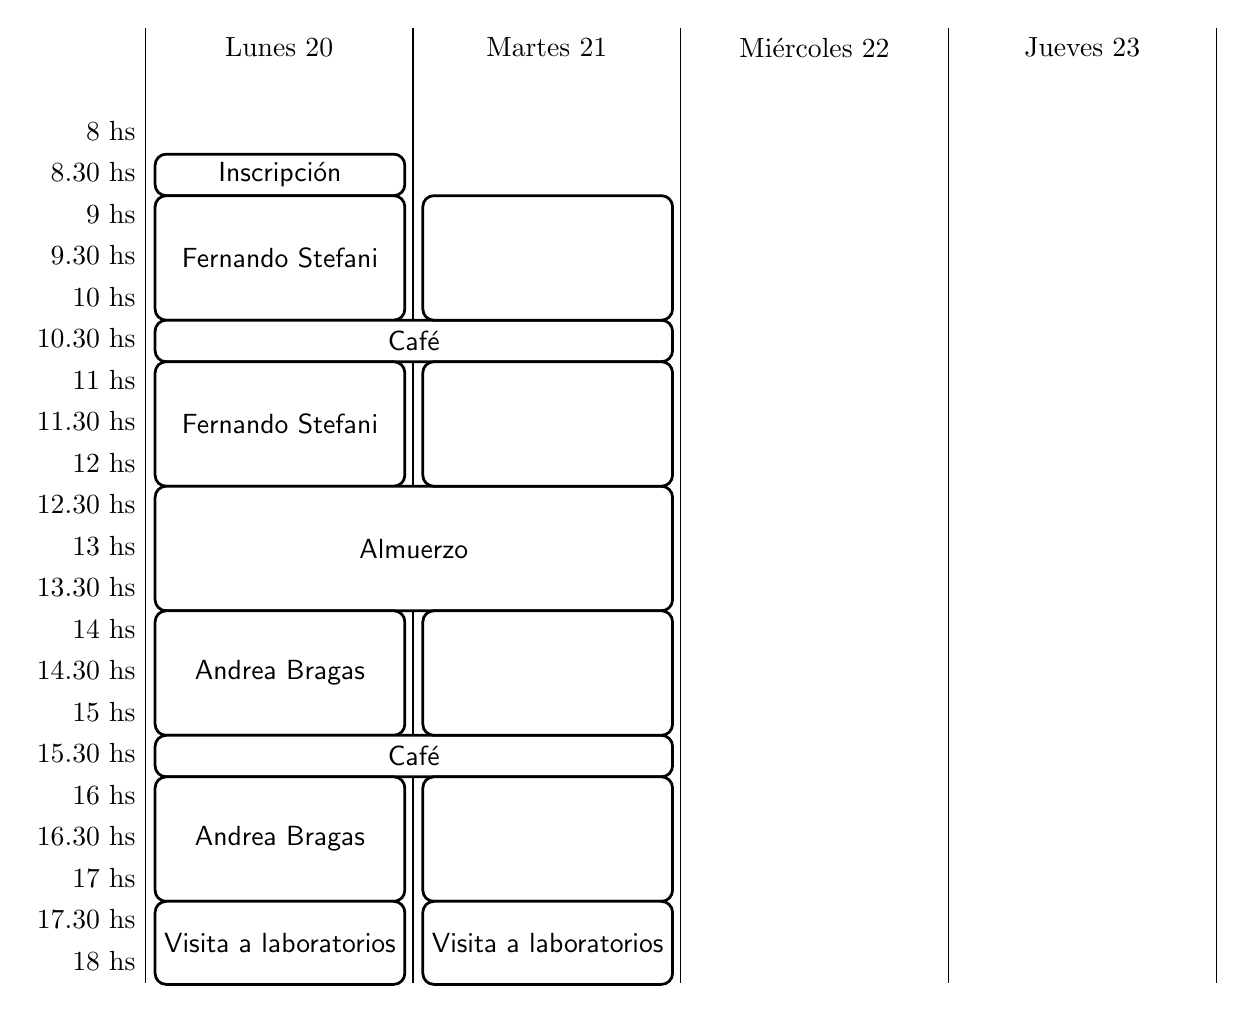
\begin{tikzpicture}[y=-\hourheight,x=\daywidth]

    % First print a list of times.
    \foreach \time/\ustime in {8/8am,9/9am,10/10am,11/11am,12/12pm,13/1pm,14/2pm,15/3pm,16/4pm,17/5pm,18/6pm}
        \node[anchor=north east] at (1,\time) {\time~hs};

    \foreach \time/\ustime in {8.30/8.30am,9.30/9.30am,10.30/10.30am,11.30/11.30am,12.30/12.30am,13.30/1.30pm,14.30/2.30pm,15.30/3.30pm,16.30/4.30pm,17.30/5.30pm}
        \node[anchor=north east] at (1,\time+0.2) {\time~hs};        
        
    % Draw some day dividers.
    \draw (1,7) -- (1,18.5);
    \draw (2,7) -- (2,18.5);
    \draw (3,7) -- (3,18.5);
    \draw (4,7) -- (4,18.5);
    \draw (5,7) -- (5,18.5);

    % Start Monday.
    \node[anchor=north] at (1.5,7) {Lunes 20};
    % Write the entries. Note that the x coordinate is 1 (for Monday) plus an
    % appropriate amount of shifting. The y coordinate is simply the starting
    % time.
    \node[entry={0.5}{1}] at (1,8.5) {Inscripci\'on};
    \node[entry={1.5}{1}] at (1,9) {Fernando Stefani};
    \node[entry={0.5}{0.5}] at (1,10.5) {Caf\'e};
    \node[entry={1.5}{1}] at (1,11) {Fernando Stefani};
    \node[entry={1.5}{0.5}] at (1,12.5) {Almuerzo};
    \node[entry={1.5}{1}] at (1,14) {Andrea Bragas};
    \node[entry={0.5}{0.5}] at (1,15.5) {Caf\'e};
    \node[entry={1.5}{1}] at (1,16) {Andrea Bragas};
    \node[entry={1}{1}] at (1,17.5) {Visita a laboratorios};
  
    
    % The same for Tuesday.
    \node[anchor=north] at (2.5,7) {Martes 21};
    \node[entry={1.5}{1}] at (2,9) {};
    \node[entry={1.5}{1}] at (2,11) {};
    \node[entry={1.5}{1}] at (2,14) {};
    \node[entry={1.5}{1}] at (2,16) {};
    \node[entry={1}{1}] at (2,17.5) {Visita a laboratorios};
    

    \node[anchor=north] at (3.5,7) {Mi\'ercoles 22};
    
    \node[anchor=north] at (4.5,7) {Jueves 23};

\end{tikzpicture}

%\end{landscape}